% =====================================================================
%  c28 —— 原文印刷页 236--242（PDF 第 237--243 页）
%  含：附录 K 的 K.1 群胚、K.2 张量范畴（K.2.1 分次向量空间、K.2.2 群的表示范畴），
%      附录 L 的开头（L. Bordism；L.1 无向配边、L.2 配边范畴、L.3 有向配边范畴）；
%      插图 Fig. 39。
%  编号公式：K.37--K.52、L.1--L.6，共 22 条。
%  说明：work/chunks/c28.txt 的文本层与本片段页码不符（其内容自印刷页 243 起，
%  实为下一片段的转储），故本片段全部内容一律以 150 dpi 页面图像为准。
% =====================================================================

\begin{figure}[htbp]
  \centering
  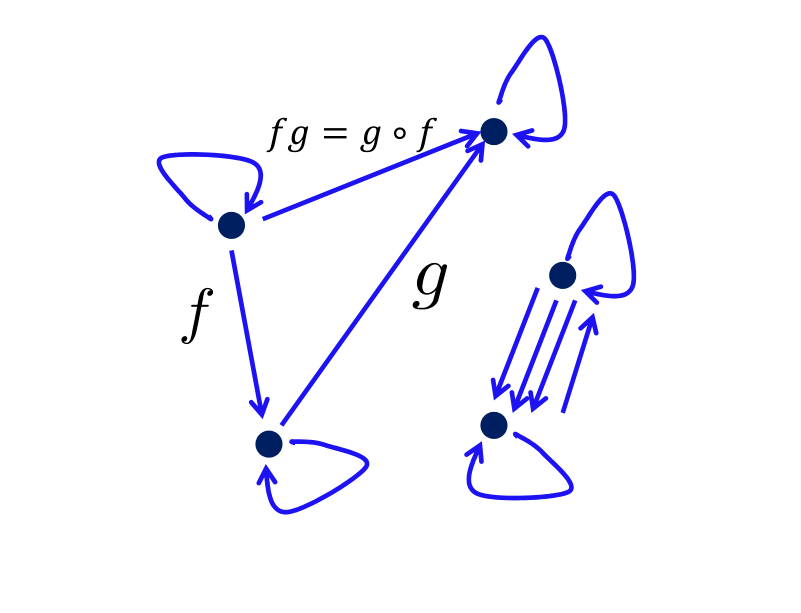
\includegraphics[width=0.55\textwidth]{figures/fig39.png}
  \caption{范畴的图示。对象是图中的黑点；图中画出了各条箭头，而人们必须给出一个规则，
    把每个箭头与别的箭头复合，并把复合的结果与某个箭头等同起来。例如，给定记作 $f$ 与 $g$
    的两个箭头，就必然存在一个形如 $f\circ g$ 的箭头。注意每个对象 $x$ 至少有一条箭头，
    即 $\operatorname{Hom}(x,x)$ 中的恒等箭头。（原文 Fig.~39，第 236 页）}
  \label{fig:39}
\end{figure}

为了看出这与我们先前关于群的概念是等价的，我们给每个态射配上一个群元素。态射的复合就是群的乘法，而态射的可逆性就是逆元素的存在性。

我们将简要描述这一观点所提供的、关于群的一个重要的、影响深远的推广。然后我们将说明，这一观点会导向一个漂亮的几何构造，它使群上同调（group cohomology）的公式变得稍微更直观一些。

\subsection{群胚} % 原文: K.1 Groupoids

\textbf{定义}\quad 一个\emph{群胚}（groupoid）是所有态射都可逆的范畴。

注意，对群胚中的任何对象 $x$，$\hom(x,x)$ 都是一个群，称为对象 $x$ 的\emph{自同构群}（automorphism group）。

\textbf{例 1}\quad 集合 $X$ 上的任何等价关系都定义一个群胚。其对象是 $X$ 的元素。若 $a\sim b$，则集合 $\hom(a,b)$ 恰有一个元素，否则为空集。态射的复合律于是意味着：$a\sim b$ 且 $b\sim c$ 蕴含 $a\sim c$。显然，每个态射都可逆。

% [Tutor Note: 「群胚」（groupoid）也有「广群」这一旧译，本译本统一用「群胚」，与 c27 一致。
% 定义处最易误读的一点是：群胚\emph{不是}群。$\hom(x,x)$ 只是对象 $x$ 的自同构群，不同对象之间的
% $\hom(x,y)$ 一般非空，故不能把整个群胚当成一个群来「乘」。例 3 正是这一区别的实例：
% 基本群胚 $\pi_{\le1}(X)$ 的对象是 $X$ 的\emph{所有}点，而基本群 $\pi_1(X,x)$ 只是其中某个
% $\hom(x,x)$；把两者混为一谈，就会误以为 $\pi_{\le1}(X)$ 依赖于基点的选取。]

\textbf{例 2}\quad 考虑量子力学中哈密顿量含时的时间演化。谈论演化算符 $U(t)$ 是没有意义的；人们必须谈论满足 $U(t_1,t_2)U(t_2,t_3)=U(t_1,t_3)$ 的酉演化 $U(t_1,t_2)$。给定 Schrödinger 方程的一个解 $\Psi(t)$，我们可以把态矢量 $\Psi(t)$ 视为对象，把 $U(t_1,t_2)$ 视为态射。这样，Schrödinger 方程的一个解就定义了一个群胚。

{\small\itshape ［原文标记：需要澄清这段话。］}
% [原文待办标记，原文 p.236 右侧页边注：\ensuremath{\clubsuit}Clarify this remark.\ensuremath{\clubsuit}]

\textbf{例 3}\quad 设 $X$ 是拓扑空间。基本群胚（fundamental groupoid）$\pi_{\le 1}(X)$ 是这样一个范畴：其对象是点 $x\in X$，其态射是道路 $f:x\to x'$ 的同伦类。这些态射按自然的方式复合。注意，点 $x\in X$ 的自同构群，即 $\hom(x,x)$，就是以 $x$ 为基点的 $X$ 的基本群 $\pi_1(X,x)$。

\textbf{例 4}\quad 规范场论：对象 = 主丛上的联络；态射 = 规范变换。对于理解超引力与弦论中出现的、由更高次微分形式构成的某些更奇特的（阿贝尔）规范场论来说，这是正确的观点。

\textbf{例 5}\quad 在弦论的轨道流形（orbifold）与 orientifold 理论中，时空必须被视为一个群胚。设 $G$ 右作用在集合 $X$ 上，于是有一个映射
\begin{equation}
  \Phi:X\times G\to X
  \tag{K.37}
  \label{eq:K.37}
\end{equation}
使得
\begin{equation}
  \Phi(\Phi(x,g_1),g_2)=\Phi(x,g_1g_2)
  \tag{K.38}
  \label{eq:K.38}
\end{equation}
\begin{equation}
  \Phi(x,1_G)=x
  \tag{K.39}
  \label{eq:K.39}
\end{equation}
对一切 $x\in X$ 与 $g_1,g_2\in G$ 成立。为简短起见，我们直接写 $\Phi(x,g):=x\cdot g$。于是可以构造范畴 $X/\!/G$，其中
\begin{equation}
\begin{split}
  \mathit{Ob}(X/\!/G) &= X\\
  \mathit{Mor}(X/\!/G) &= X\times G
\end{split}
\tag{K.40}
\label{eq:K.40}
\end{equation}
我们应当把态射想成一条以 $g$ 标记的箭头，把点 $x$ 连到点 $x\cdot g$。靶映射与源映射为
\begin{equation}
  p_0((x,g)):=x\cdot g \qquad p_1((x,g)):=x
  \tag{K.41}
  \label{eq:K.41}
\end{equation}

{\small\itshape ［原文标记：此处需要插图！］}
% [原文待办标记，原文 p.237 右侧页边注：\ensuremath{\clubsuit}FIGURE NEEDED HERE! \ensuremath{\clubsuit}]

态射的复合定义为
\begin{equation}
  (xg_1,g_2)\circ(x,g_1):=(x,g_1g_2)
  \tag{K.42}
  \label{eq:K.42}
\end{equation}
或者，用另一种记号（更适合右作用）：
\begin{equation}
  (x,g_1)(xg_1,g_2):=(x,g_1g_2)
  \tag{K.43}
  \label{eq:K.43}
\end{equation}
注意 $(x,1_G)\in\hom(x,x)$ 是恒等态射；而态射的复合之所以有意义，正是因为我们有一个群作用。还要注意，$\mathrm{pt}/\!/G$（其中 $G$ 平凡地作用在一个点上）把群 $G$ 实现为一个范畴，如上文所勾勒。

% [Tutor Note: (K.42) 与 (K.43) 是同一复合律的两种写法，但\emph{字的左右次序相反}：
% (K.42) 用熟悉的 $\circ$ 记号，(xg_1,g_2)\circ(x,g_1) 表示先走 $g_1$、再走 $g_2$，
% 即「$\circ$ 右边先作用」；(K.43) 改用并置，写成 (x,g_1)(xg_1,g_2)，把先作用的 $g_1$ 放在
% 左边。抄写或编程时若把两式的次序对齐错，会得到 $g_1g_2$ 与 $g_2g_1$ 互换的错误复合
% （对非阿贝尔 $G$，这不是小错）。核对办法：代入 $g_1=1_G$，两式都应退化为恒等态射。]

% 转写说明：例 5 与例 6 的首句在原文中逐字相同（原文 p.237），例 6 只剩这一句、
% 没有下文，显然是作者原稿中复制粘贴留下的残句。此处照录，不作合并；读者理解例 6 时
% 应把例 5 的全部内容（含 (K.37)--(K.43)）算作它的正文。

\textbf{例 6}\quad 在弦论的轨道流形与 orientifold 理论中，时空必须被视为一个群胚。（这与上一个例子密切相关。）

\medskip
\noindent\rule{\linewidth}{0.4pt}
\medskip
\noindent\textbf{练习}

设 $G$ 是一个群。我们定义一个群胚，记作 $G/\!/G$（理由见后文），其对象是群元素 $\mathit{Obj}(G/\!/G)=G$，其态射是由
\begin{equation}
  g_1\xrightarrow{\ h\ }g_2
  \tag{K.44}
  \label{eq:K.44}
\end{equation}
给出的箭头，即当且仅当 $g_2=h^{-1}g_1h$ 时才存在的箭头。这是圆周上主 $G$-丛的群胚。

画出对应于 $S_3$ 的群胚。

\subsection{张量范畴} % 原文: K.2 Tensor Categories

为了定义 TFT，我们需要张量范畴（tensor category）这一进一步的概念。注意，给定一个范畴 $C$，笛卡尔积 $C\times C$、$C\times C\times C$、…… 也按自然的方式成为范畴。

\textbf{定义}\quad 一个\emph{张量范畴}（tensor category，也称\emph{幺半范畴} monoidal category）是带有一个函子 $\otimes:C\times C\to C$ 的范畴，使得两个函子 $\otimes\circ\otimes_{12}:C\times C\times C\to C$ 与 $\otimes\circ\otimes_{23}:C\times C\times C\to C$ 之间存在一个同构 $\mathcal{A}$ 满足五边形公理（pentagon identity），并且存在一个单位对象（identity object）$1_C$，连同函子 $C\to C$ 之间的自然变换
\begin{equation}
  \iota_L:1_C\otimes\cdot\ \to\mathrm{Id}
  \tag{K.45}
  \label{eq:K.45}
\end{equation}
\begin{equation}
  \iota_R:\cdot\otimes 1_C\to\mathrm{Id}
  \tag{K.46}
  \label{eq:K.46}
\end{equation}
这些数据还需服从若干自然的相容性条件：

{\small\itshape ［原文标记：我们是否要求对偶对象存在？］}
% [原文待办标记，原文 p.238 右侧页边注：\ensuremath{\clubsuit}Do we require the existence of a dual object?\ensuremath{\clubsuit}]

为举例说明这些相容性条件，我们考虑关于自然变换 $\mathcal{A}$ 的第一个条件：对 $C_0$ 中的一切对象 $x,x',x''$，有一个同构
\begin{equation}
  \mathcal{A}_{x,x',x''}:(x\otimes x')\otimes x''\to x\otimes(x'\otimes x'')
  \tag{K.47}
  \label{eq:K.47}
\end{equation}
它满足五边形公理：

% 转写说明：主文件未载入绘图宏包，故五边形交换图用 array 排布；五个顶点、五条箭头的
% 方向与原文 p.238 的图一致（上行的水平箭头、两侧的斜箭头，以及底部汇合的斜箭头）。

{\small
\begin{equation}
\begin{array}{ccc}
\big((x_1\otimes x_2)\otimes x_3\big)\otimes x_4 & \longrightarrow &
\big(x_1\otimes x_2\big)\otimes\big(x_3\otimes x_4\big)\\[10pt]
\swarrow & & \searrow\\[10pt]
\big(x_1\otimes(x_2\otimes x_3)\big)\otimes x_4 & &
x_1\otimes\big(x_2\otimes(x_3\otimes x_4)\big)\\[10pt]
\searrow & & \nearrow\\[10pt]
& x_1\otimes\big((x_2\otimes x_3)\otimes x_4\big) &
\end{array}
\tag{K.48}
\label{eq:K.48}
\end{equation}
}

{\small\itshape ［原文标记：修正 $xy$ 矩阵。］}
% [原文待办标记，原文 p.238 右侧页边注：\ensuremath{\clubsuit}FIX xy matrix \ensuremath{\clubsuit}，紧挨着上面的五边形图；
% 所指应是图中 $x_1,\dots,x_4$ 的下标排布（或图中箭头的 $x,y$ 记号），原意不明，照录。]

于是有定理（“相干定理”，coherence theorem）：无论怎样加括号，$x_0\otimes x_1\otimes\cdots\otimes x_n$ 在相差同构的意义下都是良定义的。关于自然变换 $\iota_L$ 与 $\iota_R$ 的条件则相当显然。

\textbf{例}\quad 范畴 $\mathbf{VECT}_\kappa$ 是张量范畴。张量单位 $1_{\mathbf{VECT}_\kappa}$ 是什么？

设 $\sigma:C\times C\to C\times C$ 是交换函子（exchange functor），它在对象与态射上交换两个因子。

\textbf{定义}\quad 一个\emph{对称幺半范畴}（symmetric monoidal category）是带有一个同构 $\Omega$ 的幺半范畴，该 $\Omega$ 是 $\otimes\circ\sigma$ 与 $\otimes$ 之间的同构，且其平方为恒等。同样，它与 $\mathcal{A}$、$\iota_L$、$\iota_R$ 之间有许多相当显然的相容性条件。

这仍然意味着，对一切对象 $x,y$ 都有同构
\begin{equation}
  \Omega_{x,y}:x\otimes y\to y\otimes x
  \tag{K.49}
  \label{eq:K.49}
\end{equation}
使得 $\Omega_{y,x}\circ\Omega_{x,y}=1_{x\otimes y}$。

% [Tutor Note: 定义里要求的是「自然变换」$\iota_L,\iota_R$，而 (K.45)(K.46) 又额外说它们
% 是「同构」——两件事不能混：自然变换只需要每个分量 $(\iota_L)_x:1_C\otimes x\to x$ 存在并与
% 态射相容，而同构还要求每个分量可逆。张量范畴的公理必须\emph{同时}给出结合子 $\mathcal{A}$
% (K.47) 与左右单位子 (K.45)(K.46)；相干定理的作用正是保证只需验证五边形公理 (K.48) 与
% 三角形公理，而不必逐一验证「任意加括号方式的复合都相等」这无穷多条等式。作者的
% "fairly obvious" 指的就是三角形公理那一条，原文未写出，读者可自行补出：
% $(x\otimes 1_C)\otimes y\xrightarrow{\ \mathcal{A}\ }x\otimes(1_C\otimes y)
% \xrightarrow{\ 1\otimes\iota_L\ }x\otimes y$ 应等于 $\iota_R\otimes 1$。
% 术语取舍：原文在定义张量范畴时明说 "also known as a monoidal category"，
% 即把 tensor category 与 monoidal category 当作同义词；但严格说这是两个层次——monoidal
% 只要求 (K.45)--(K.48) 这一套（结合子、单位子、五边形、三角形），symmetric 则是在此之上
% 再加一个平方为 $1$ 的 $\Omega$ (K.49)。本译本按原文把前者译「张量范畴/幺半范畴」、
% 后者译「对称幺半范畴」；读文献时若见到 "tensor category" 指「带刚性（对偶）的对称
% 幺半范畴」（如 Deligne--Milne 的用法），要按上下文判断，不能一律套用本节定义。
% 紧接着引入的 braided（编织）是本书反复用到的概念（任意子的编织），务必与 symmetric 区分：
% 编织只要求 $\Omega$ 可逆，\emph{不}要求 $\Omega^2=1$；$\Omega^2=1$ 的编织范畴正是对称
% 幺半范畴。$2+1$ 维任意子的统计相位一般不为 $\pm1$，所以物理上真正需要的是编织而非对称
% ——这正是作者在此处把它作为「重要推广」引入的原因。]

\textbf{注}\quad 对共形场论以及 $2+1$ 维中的准粒子统计而言，一个重要推广是\emph{编织张量范畴}（braided tensor category）的概念：其中仍有同构 $\Omega$，但它的平方不为 $1$。

最后，我们需要（对称）张量函子（tensor functor）这一记号。它是两个对称张量范畴之间的函子 $F:C\to D$，连同同构 $1_D\to F(1_C)$，以及两个函子 $C\times C\to D$（分别由 $F\circ\otimes$ 与 $\otimes\circ F\times F$ 给出）之间的一个同构。

\subsubsection{$\mathbb{Z}_2$ 分次向量空间} % 原文: K.2.1 Z2-graded vector spaces

一个 $\mathbb{Z}_2$ 分次向量空间是带有分解 $V=V_0\oplus V_1$ 的向量空间，其中下标被理解为 $\mathbb{Z}_2$ 的元素。在 $\mathbb{Z}_2$ 分次向量空间的范畴中，我们可以引入两种不同的张量范畴。对于 $\mathbb{Z}_2$ 分次向量空间，我们能够并且将会使用分次张量积（graded tensor product）。此时有同构
\begin{equation}
  \Omega:V\otimes W\to W\otimes V
  \tag{K.50}
  \label{eq:K.50}
\end{equation}
但必须小心地运用 Koszul 符号规则：若 $v,w$ 是齐次元素，则
\begin{equation}
  \Omega(v\otimes w)=(-1)^{|v|\cdot|w|}\,w\otimes v
  \tag{K.51}
  \label{eq:K.51}
\end{equation}
这条规则有一个重要推论：如果我们有任何一族超向量空间（supervector space）$(V_\alpha)_{\alpha\in I}$（其中下标 $\alpha$ 标记不同的超向量空间，不应与 $\mathbb{Z}_2$ 分次混淆），那么就存在唯一一个典范的张量积
\begin{equation*}
  \bigotimes_{\alpha}V_\alpha
\end{equation*}
而无需指定任何次序。

% [Tutor Note: (K.51) 的符号因子指数是 $|v|\cdot|w|$，其中 $|v|,|w|\in\{0,1\}$ 是
% $\mathbb{Z}_2$ 次数（\emph{不是} $\mathbb{Z}$-次数，也不是 $V$ 的维数）。两个奇元素交换
% 两次给出 $(-1)^{1\cdot1}\cdot(-1)^{1\cdot1}=+1$，故交换子平方为恒等；而两个奇元素之间的
% 一次交换给出 $-1$（交换两次才回到原状），这正是「典范张量积无需指定次序」的来源：换序
% 至多差一个由次数决定的符号，而这个符号不依赖于换序的路径。抄写时最易把
% $(-1)^{|v||w|}$ 写成 $(-1)^{|v|+|w|}$，后者对两个奇元素给出 $+1$，与超代数约定相反。]

\subsubsection{群的表示范畴} % 原文: K.2.2 Category Of Representations Of A Group

设 $G$ 是一个群。那么存在一个范畴，其对象是表示，态射是表示之间的缠结算子（intertwiner），即与 $G$ 的作用交换的表示之间的映射。

现在设 $G$ 是紧群，并限制到有限维表示的子范畴。记之为 $\mathrm{Rep}(G)$。这是一个张量范畴。此外，有一组“单”对象，即不可约表示 $V_\lambda$，使得所有对象都同构于单对象的直和。张量函子由“融合规则”（fusion rules）
\begin{equation}
  V_\lambda\otimes V_\mu\cong D^\rho_{\lambda\mu}\otimes V_\rho
  \tag{K.52}
  \label{eq:K.52}
\end{equation}
决定，其中 $D^\rho_{\lambda\mu}$ 是描述简并的有限维实向量空间。

% [Tutor Note: (K.52) 照原文转写，但它用的是对 $\rho$ 的隐式求和并省略了直和号；
% 通常的写法是 $V_\lambda\otimes V_\mu\cong\bigoplus_\rho D^\rho_{\lambda\mu}\otimes V_\rho$，
% 其中 $D^\rho_{\lambda\mu}$ 是多重数空间，$\dim D^\rho_{\lambda\mu}=N^\rho_{\lambda\mu}$
% 即融合系数（非负整数）。若把 (K.52) 当等式逐项读而不求和，就会得出「两个不可约表示的
% 张量积仍是不可约的」这一错误结论——只有 $G=U(1)$ 这类情形才对。]

\section{配边} % 原文: L. Bordism

\begin{keytakeaways}
  \item 配边的定义 \eqref{eq:L.1}：从闭 $(d-1)$ 维流形 $Y_0$ 到 $Y_1$ 的配边是一个 $d$ 维流形 $X$，
    其边界被不交地划分为 $(\partial X)_0\sqcup(\partial X)_1$，并带有从边界「领」（collar）
    $[0,1)\times Y_0$、$(-1,0]\times Y_1$ 到 $X$ 的嵌入 $\theta_0,\theta_1$；这些额外数据的作用
    正是使粘合（gluing）有定义。
  \item 群结构：不交并给出 $n$ 维流形配边等价类 $\Omega_n$ 上的阿贝尔群结构，空集 $\varnothing^n$
    是零元；$[0,1]\times X$ 给出 $X\sqcup X$ 与 $\varnothing$ 的配边，故 $2[X]=0$，每个元素都是二阶的。
  \item 低维计算：$\Omega_0\cong\mathbb{Z}/2\mathbb{Z}$（两个点零配边）、$\Omega_1=0$（圆周是圆盘的边界）、
    $\Omega_2\cong\mathbb{Z}/2\mathbb{Z}$（生成元 $[\mathbb{RP}^2]$，用 Euler 示性数的奇偶性论证）。
  \item Thom 定理 \eqref{eq:L.2}：$\Omega_*\cong R[x_2,x_4,x_5,\dots]$，$R=\mathbb{Z}/2\mathbb{Z}$，
    $k$ 次生成元 $x_k$ 恰有一个，且只对 $k\ne 2^j-1$ 出现；偶次生成元是 $\mathbb{RP}^k$ 的配边类。
  \item 范畴化：$\mathrm{Bord}_{\langle d-1,d\rangle}$ 以闭 $(d-1)$ 维流形为对象、配边的同胚类为态射，
    复合是粘合，它是对称张量范畴（不交并为张量积、空流形为单位）；有向版本见第 L.3 小节，
    它要求边界嵌入保定向，并给出对偶配边 $X^\vee:Y_1^\vee\to Y_0^\vee$。
\end{keytakeaways}

这一数学主题是拓扑场论的重要背景。关于该主题有一本经典著作：
\begin{quote}
Milnor and Stasheff, \emph{Characteristic Classes}, PUP\\
更技术性的细节可在 R. Stong 的书中找到。\\
此外，我们还使用了 Dan Freed 那份非常好的讲义中的一些材料：\\
D. Freed, ``Bordism Old And New,''\\
\url{https://www.ma.utexas.edu/users/dafr/M392C-2012/index.html}
\end{quote}

\subsection{无向配边：定义与例子} % 原文: L.1 Unoriented Bordism: Definition And Examples

下面给出配边（bordism）的正式定义：

\textbf{定义}\quad 设 $Y_0,Y_1$ 是两个闭的 $(d-1)$ 维流形。从 $Y_0$ 到 $Y_1$ 的一个\emph{配边}是
\begin{enumerate}
  \item 一个 $d$ 维流形 $X$，连同其边界的一个不交划分
  \begin{equation}
    \partial X=(\partial X)_0\sqcup(\partial X)_1
    \tag{L.1}
    \label{eq:L.1}
  \end{equation}
  \item 一对嵌入 $\theta_0:[0,1)\times Y_0\to X$ 与 $\theta_1:(-1,0]\times Y_1\to X$，它们是到其像上的微分同胚，并且使得限制 $\theta_0:\{0\}\times Y_0\to(\partial X)_{\mathrm{in}}$ 与 $\theta_1:\{0\}\times Y_1\to(\partial X)_{\mathrm{out}}$ 都是同胚。
\end{enumerate}

与我们先前所说的相比，这个定义之所以多出一层复杂性，是因为这些额外的数据便于把配边粘合起来产生新的配边。

容易看出，配边是一个等价关系；而不交并（disjoint union）在 $n$ 维流形的配边等价类空间 $\Omega_n$ 上定义一个阿贝尔群结构。该群的零元素是空集 $\varnothing^n$ 的等价类；任何闭 $n$ 维流形 $X$ 都是自己的逆元，因为 $[0,1]\times X$ 可以看作 $X\sqcup X$ 与 $\varnothing$ 之间的一个配边。于是在 $\Omega_n$ 中 $2[X]=0$。

\textbf{例}

\begin{enumerate}
  \item 只有一种非平凡的零维流形，即点；而我们刚刚看到，两个点的不交并是零配边的，因此 $\Omega_0\cong\mathbb{Z}/2\mathbb{Z}$。注意，若去掉对 $X$ 的流形条件，那么字母 Y（即 Y 形的空间）就会给出两个点（等价于零）与一个点之间的一个配边，于是配边群将是平凡的。因此，流形条件是重要的。
  \item $\Omega_1=0$，因为唯一的闭连通一维流形是圆周，而它显然是一个圆盘的边界。
  \item 可以证明 $\Omega_2\cong\mathbb{Z}/2\mathbb{Z}$，生成元是 $[\mathbb{RP}^2]$。其论证如下（取自 D. Freed 的讲义 ``Bordism Old And New,'' 见其主页）。紧曲面的分类表明，曲面由两个不变量刻画：可定向性与 Euler 示性数。可定向曲面显然零配边。请注意！Euler 示性数\emph{不是}配边不变量！不可定向曲面都可由与 $\mathbb{RP}^2$ 作连通和得到。两个 $\mathbb{RP}^2$ 的连通和是圆周上的圆丛。取 $[0,1]\times S^1$ 并按 $\{(0,z)\}\sim\{(1,\bar z)\}$ 作商（其中把 $S^1$ 视为单位复数）。注意，我们可以把 $S^1$ 换成圆盘 $D^2$，并用同样的等同 $\{(0,z)\}\sim\{(1,\bar z)\}$ 得到从 Klein 瓶到零的一个配边。下面我们断言，$\mathbb{RP}^2$ 给出一个非平凡的配边类。因为，若它有一个到零的配边、即 $\partial X=\mathbb{RP}^2$，则对 $X$ 作三角剖分就给出双倍 $X\cup_{\mathbb{RP}^2}X$ 的一个三角剖分，其 Euler 示性数为 $2\chi(X)-1$。另一方面，闭三维流形的 Euler 示性数为零。现在，一般的连通不可定向曲面是 $n$ 个 $\mathbb{RP}^2$ 的连通和。把它们两两分组，并为每一对取一个到零的配边，就可以把配边类等同于 $\mathbb{Z}/2\mathbb{Z}$ 中的元素 $n\bmod 2$。
  \item 为描述全部配边群 $\Omega_d$，有用的一点是注意到流形的笛卡尔积与配边等价关系相容，这使得 $\Omega_*\cong\bigsqcup_{d\ge 0}\Omega_d$ 成为一个 $\mathbb{Z}$-分次环，分次由维数给出。Thom 证明了
  \begin{equation}
    \Omega_*\cong R[x_2,x_4,x_5,x_6,x_8,x_9,x_{10},x_{11},x_{12},x_{13},x_{14},x_{16},x_{17},\dots]
    \tag{L.2}
    \label{eq:L.2}
  \end{equation}
  其中 $R=\mathbb{Z}/2\mathbb{Z}$，并且只要 $k$ 不是 $2^j-1$ 的形式，就恰有一个 $k$ 次生成元 $x_k$。偶次生成元是 $\mathbb{RP}^k$ 的配边类，奇次生成元则是 $(S^m\times\mathbb{CP}^\ell)/\mathbb{Z}_2$ 的一个商，其中 $\mathbb{Z}_2$ 的作用是（对径映射，复共轭）。
  \item 此外，对任何流形都有一系列上同调类 $w_i(Y)\in H^i(Y;\mathbb{Z}/2\mathbb{Z})$，称为 Stiefel-Whitney 类。它们与切丛的扭曲（twisting）相关联。（例如，$w_1(Y)$ 刻画 $Y$ 是否可定向。）一个流形的\emph{Stiefel 数}是 $\mathbb{Z}/2\mathbb{Z}$ 中元素构成的序列
  \begin{equation}
    \langle w_{i_1}(Y)\cup\cdots\cup w_{i_k}(Y),[Y]\rangle
    \tag{L.3}
    \label{eq:L.3}
  \end{equation}
  而两个流形配边，当且仅当它们的全部 Stiefel 数都相同。关于最后两项，参见 Milnor 与 Stasheff 的优秀著作 \emph{Characteristic Classes}。\footnote{如果我们讲到特征类那一章，就会证明这两个结果。}
\end{enumerate}

% [Tutor Note: 第 3 条从「$X\cup_{\mathbb{RP}^2}X$ 的 Euler 示性数为 $2\chi(X)-1$」到矛盾，
% 缺了一步：双倍公式应为 $\chi(\text{double})=2\chi(X)-\chi(\mathbb{RP}^2)$，而
% $\chi(\mathbb{RP}^2)=1$，故该数为奇数；闭三维流形的 Euler 示性数为 $0$（偶数），矛盾。
% 作者省略了「$\chi(\mathbb{RP}^2)=1$」与「奇数不等于零」这两小步。另注意本段用的
% Euler 示性数对带边流形也成立（拓扑不变量），无需可定向性，这正是论证能用于不可定向曲面的原因。]

\subsection{配边范畴 $\mathrm{Bord}_{\langle d-1,d\rangle}$} % 原文: L.2 The Bordism Category Bord$\langle d-1,d\rangle$

现在我们可以定义一个\emph{配边范畴} $\mathrm{Bord}_{\langle d-1,d\rangle}$。
\begin{enumerate}
  \item 对象：闭的 $(d-1)$ 维流形，通常记作 $Y$。
  \item $\hom(Y_0,Y_1)$ 是配边 $X:Y_0\to Y_1$ 的同胚类的集合。配边 $X$ 与 $X'$ 之间的一个同胚，是带边流形之间的同胚，它把 $(\partial X)_{\mathrm{in}}$ 送到 $(\partial X')_{\mathrm{in}}$，并与领 $\theta_0,\theta_1$ 交换。
\end{enumerate}

配边范畴中态射的复合通过粘合实现。由于我们按同胚来等同配边，配边 $X=[0,1]\times Y$（从 $Y$ 到 $Y$）就是恒等态射 $1_Y$。范畴 $\mathrm{Bord}_{\langle d-1,d\rangle}$ 是一个对称张量范畴：张量积是不交并，而空流形 $\varnothing^{d-1}$ 是张量单位。

% [Tutor Note: 范畴约定：这里的态射是配边的\emph{同胚类}，不是微分同胚类——无向配边
% 范畴根本不带光滑结构，「微分同胚」无从谈起；到了有向情形 (L.3)，才改用保定向的
% \emph{微分同胚}来等同。两处若混用，粘合的定义与恒等态射 $1_Y=[0,1]\times Y$ 的验证都会
% 出问题（例如 $[0,1]\times Y$ 与 $[0,2]\times Y$ 只在同胚意义下相同，而非微分同胚意义下
% 逐点相同）。另外注意「领」（collar）$\theta_0,\theta_1$ 是态射数据的一部分：没有它，
% 粘合只能定义到同胚为止，复合的结合律无法直接验证。]

\subsection{有向配边范畴 $\mathrm{Bord}^{\mathrm{SO}}_{\langle d-1,d\rangle}$} % 原文: L.3 The Oriented Bordism Category Bord$^{SO}_{\langle d-1,d\rangle}$

我们常常关心\emph{有向配边}（oriented bordism）。

为了定义有向配边，我们对配边的定义略作修改。现在 $Y_0,Y_1,X$ 都是定向的。嵌入 $\theta_0$ 与 $\theta_1$ 要求保持定向，并且我们按定向微分同胚来等同配边 $X$ 与 $X'$。

$\theta_0$ 与 $\theta_1$ 保持定向这一条件必须小心处理。注意，如果给定若干定向实向量空间的一个和，那么直和上并没有自然的定向。然而，如果给定一个正合序列
\begin{equation}
  0\to V_1\to V_2\to V_3\to 0
  \tag{L.4}
  \label{eq:L.4}
\end{equation}
那么就有一个典范同构 $\operatorname{DET}V_3\cong\operatorname{DET}V_1\to\operatorname{DET}V_2$；因此，若三个空间中有两个已定向，我们便可要求这个典范同构保持定向，从而确定第三个空间的定向。特别地，子流形与外围流形上的定向确定了法丛上的定向。在定义 $\theta_0$、$\theta_1$ 时，我们用 $\mathbb{R}$ 上的标准定向 $+\partial/\partial x$ 来定向 $[0,+1)$ 与 $(-1,0]$，然后取 $[0,+1)\times Y$ 与 $(-1,0]\times Y$ 上的乘积定向。

% [Tutor Note: 原文 (L.4) 之后印作 $\operatorname{DET}V_3\cong\operatorname{DET}V_1\to
% \operatorname{DET}V_2$，箭头处应是 $\otimes$：正合序列 $0\to V_1\to V_2\to V_3\to0$ 给出
% 行列式线丛的乘法性 $\operatorname{DET}V_2\cong\operatorname{DET}V_1\otimes
% \operatorname{DET}V_3$（等价地 $\operatorname{DET}V_3\cong\operatorname{DET}V_1\otimes
% \operatorname{DET}V_2$，取决于 $\operatorname{DET}$ 与对偶的约定）。这是原文 p.242 的
% 排印错误（$\otimes$ 误作 $\to$），译文照录未改；核对时可验一下维数：若 $V_3=V_2/V_1$，
% 则 $\dim V_2=\dim V_1+\dim V_3$，两边行列式线丛的次数相加才对得上。]

\textbf{定义}\quad 对每个有向配边 $X:Y_0\to Y_1$，都有一个\emph{对偶有向配边} $X^\vee:Y_1^\vee\to Y_0^\vee$。让我们仔细把它写出来，因为这容易引起混淆。$Y^\vee$ 表示带相反定向的 $Y$。$X^\vee$ 是取\emph{相同}定向的流形 $X$；但我们交换入边与出边。此外，
\begin{equation}
  \theta_0^\vee(t,y_1)=\theta_1(-t,y_1) \qquad \forall t\in[0,+1)\quad\&\quad y_1\in Y_1
  \tag{L.5}
  \label{eq:L.5}
\end{equation}
\begin{equation}
  \theta_1^\vee(t,y_0)=\theta_0(-t,y_0) \qquad \forall t\in(-1,0]\quad\&\quad y_0\in Y_0
  \tag{L.6}
  \label{eq:L.6}
\end{equation}
注意，$\theta_0^\vee$ 与 $\theta_1$ 之间的关系涉及一个反转定向的变换 $t\to -t$；因此，由于 $X^\vee$ 与 $X$ 具有相同的定向，我们要求 $Y$ 上的定向也反转。若忘掉定向，我们也得到无向情形下对偶配边的概念。

再一次地，我们可以定义有向配边群 $\Omega_n^{\mathrm{SO}}$（$n\ge 0$）、有向配边环 $\Omega_*^{\mathrm{SO}}$，以及有向配边范畴 $\mathrm{Bord}^{\mathrm{SO}}_{\langle d-1,d\rangle}$。

\textbf{例 1}\quad 考虑有向配边群 $\Omega_0^{\mathrm{SO}}$。点有两种：$\mathrm{pt}_+$ 与 $\mathrm{pt}_-$；基本连通有向配边有五种，如图 40 所示。于是 $\Omega_0^{\mathrm{SO}}\cong\mathbb{Z}$。该同构取 $+$ 点数目与 $-$ 点数目的差。

\textbf{例 2}\quad 在 $1$ 维与 $2$ 维，我们同样得到零配边群。
